\begin{enumerate}[label=\thesubsection.\arabic*.,ref=\thesubsection.\theenumi]
\item In 
	\figref{fig:tri-isosc},	
\begin{figure}[H]
	\begin{center}
		{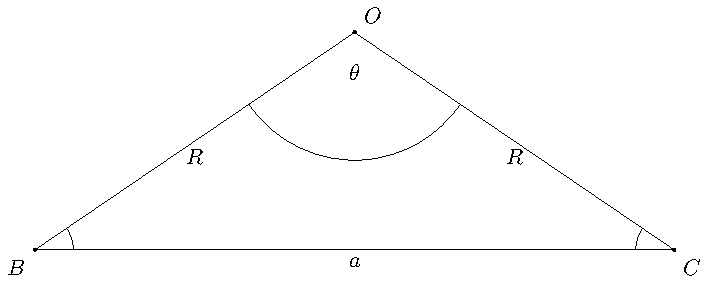
\includegraphics[width=0.6\columnwidth]{figs/trig_id/ccircle/tri_isosc.pdf}}
	\end{center}
	\caption{Isosceles Triangle}
	\label{fig:tri-isosc}	
\end{figure}
\begin{align}
	OB = OC=R
\end{align}
Such a triangle is known as an isosceles triangle.  Show that
\begin{align}
	\angle B = \angle C
\end{align}
\solution 
Using
\eqref{eq:tri_sin_form},
\begin{align}
	\frac{\sin B}{R} &= \frac{\sin C}{R}
	\\
\implies	{\sin B} &= {\sin C}
\\
	\text{or, } \angle B &= \angle C.
\end{align}
\item In 
	\figref{fig:tri-isosc},	
	show that 
  \begin{align}
	  a = 2R \sin\frac{ \theta }{2}
\label{eq:crad_cos2a}
  \end{align}
		\solution In $\triangle OBC$,  using the cosine formula from
\eqref{eq:tri_cos_form},
\begin{align}
	\cos \theta &= \frac{R^2+R^2 - a^2}{2R^2} = 1 -\frac{a^2}{2R^2}
	\\
	\implies \frac{a^2}{2R^2}&= 2\sin^2\frac{\theta}{2}
\end{align}
yielding 
\eqref{eq:crad_cos2a}.

\item In 
	\label{prob:tri-ccentre-def}
	\figref{fig:tri-perp-bis}, 
\begin{align}
OB = OC=R, 	BD = DC.
\end{align}
Show that $OD \perp BC$.
%
\begin{figure}[H]
	\begin{center}
		
		{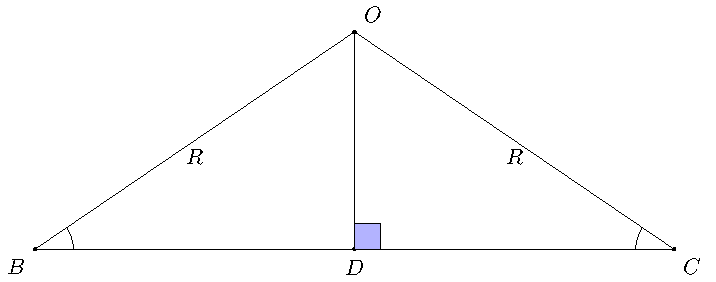
\includegraphics[width=0.6\columnwidth]{figs/trig_id/ccircle/tri-perp-bis.pdf}}
	\end{center}
	\caption{Perpendicular bisector.}
	\label{fig:tri-perp-bis}	
%github/geometrfigs/
\end{figure}
\item In 
	\figref{fig:tri_ccentre},
$OD$ and $OE$ are the perpendicular bisectors of sides $BC$ and $AC$ respectively.  Show that 
$OA = R$.
\begin{figure}[H]
	\begin{center}
		
		{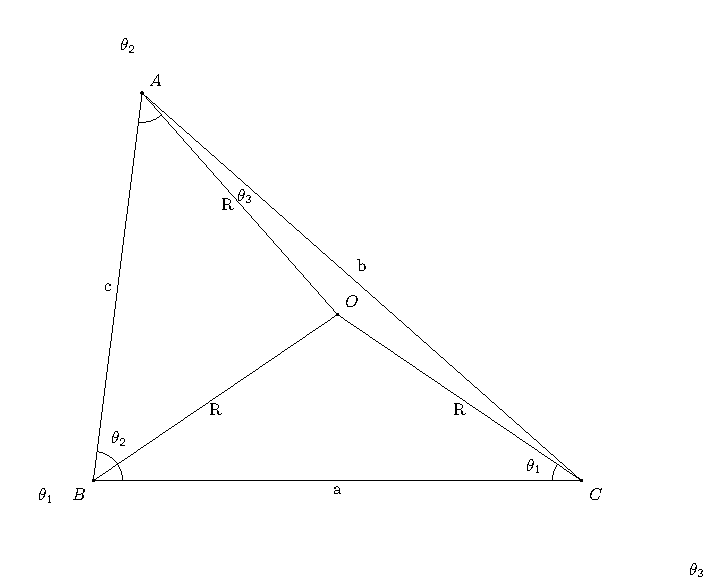
\includegraphics[width=0.6\columnwidth]{figs/trig_id/ccircle/tri_ccentre.pdf}}
	\end{center}
	\caption{ Perpendicular bisectors of $\triangle ABC$ meet at $\vec{O}$.}
	\label{fig:tri_ccentre}	
\end{figure}
\item In
	\figref{fig:tri_ccentre},
	%\figref{fig:tri_ccircle-ang},
show that 
\begin{align}
\label{eq:tri_crad_R}
\frac{a}{\sin A} = \frac{b}{\sin B} = \frac{c}{\sin C} = 2R.
\end{align}
%
%
\solution
From 
\eqref{eq:ang-subtend-ccentre}
and 
\eqref{eq:crad_cos2a}
  \begin{align}
	  a = 2R \sin A
  \end{align}
  \item 
	\figref{fig:tri_ccircle-ang}
  shows the {\em circumcircle} of $\triangle ABC$.
\begin{figure}[H]
	\begin{center}
		{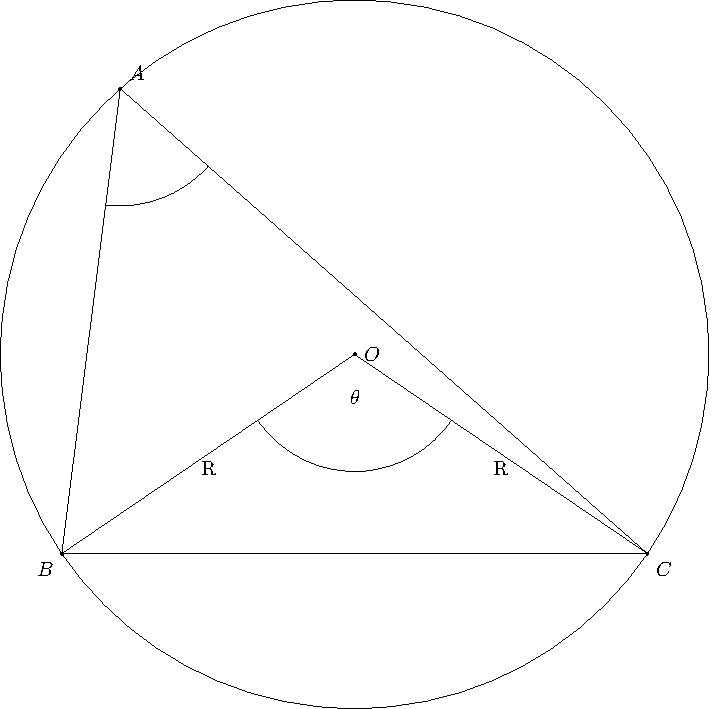
\includegraphics[width=0.6\columnwidth]{figs/trig_id/ccircle/tri_ccircle.pdf}}
	\end{center}
	\caption{Circumcircle of $\triangle ABC$}
	\label{fig:tri_ccircle-ang}	
\end{figure}
\item Any point on the circle can be expressed as 
  \begin{align}
	  \vec{x} = \vec{O} + R\myvec{\cos \theta \\ \sin \theta}, \quad 0 \in \sbrak{0, 2\pi}
\label{eq:polar-ccentre}.
  \end{align}
  where $\vec{O}$ is the centere of the circle.
  \item Let
  \begin{align}
	  R = 1,\,
	  \vec{O} = \vec{0} ,\,
	  \vec{A} = \myvec{\cos \theta_1 \\ \sin \theta_1},\,
	  \vec{B} = \myvec{\cos \theta_2 \\ \sin \theta_2},\,
  \end{align}
Show that the distance
  \begin{align}
	  AB = \norm{\vec{A}-\vec{B}} = 
	   2 \sin \brak{\frac{\theta_1-\theta_2}{2}}
\label{eq:norm-polar-ccentre}
  \end{align}
  \solution 
  From 
\eqref{eq:polar-ccentre}.
  \begin{align}
	  \vec{A}-\vec{B} &= 
\myvec{\cos \theta_1-\cos \theta_2 \\ \sin \theta_1-\sin \theta_2}
\\
\implies 
	  \norm{\vec{A}-\vec{B}}^2 &= 
	  \brak{\vec{A}-\vec{B}}^\top
	  \brak{\vec{A}-\vec{B}} 
	  \\
	  &= 
	  \brak{\cos \theta_1-\cos \theta_2}^2 +\brak{\sin \theta_1-\sin \theta_2}^2
	  \\
	  &= 2\cbrak{1-
	  \cos \brak{\theta_1-\theta_2}} = 4 \sin^2 \brak{\frac{\theta_1-\theta_2}{2}}
  \end{align}
  yielding 
\eqref{eq:norm-polar-ccentre} from
\eqref{eq:trig-id-2A-cos}.
  \item In 
	\figref{fig:tri_ccircle-ang}, show that 
\begin{align}
	\cos A = \frac{
	  \brak{\vec{A}-\vec{B}}^\top
	  \brak{\vec{A}-\vec{B}} 
}
{
	  \norm{\vec{A}-\vec{B}}
	  \norm{\vec{A}-\vec{C}}
}
\label{eq:tri_cos_form-ccentre-norm},
\end{align}
  \item In 
	\figref{fig:tri_ccircle-ang},
show that 
  \begin{align}
	  \theta = 2A
\label{eq:ang-subtend-ccentre}.
  \end{align}
The angle subtended by an arc at the centre is double the angle subtended by it at any point on the remaining part of the circle.
  \solution Let 
  \begin{align}
	  \vec{C} = \myvec{\cos \theta_3 \\ \sin \theta_3}
  \end{align}
  Then, 
  substituting 
  from 
\eqref{eq:norm-polar-ccentre}
in 
\eqref{eq:tri_cos_form},
%\eqref{eq:tri_cos_form-ccentre-norm},
  \begin{align}
	  \cos A &= \frac{4 \sin^2 \brak{\frac{\theta_1-\theta_2}{2}} +4\sin^2 \brak{\frac{\theta_1-\theta_3}{2}}-4 \sin^2 \brak{\frac{\theta_2-\theta_3}{2}}}{8 \sin \brak{\frac{\theta_1-\theta_2}{2}} \sin \brak{\frac{\theta_1-\theta_3}{2}}}
	  \\
	   &= \frac{2 \sin^2 \brak{\frac{\theta_1-\theta_2}{2}} +\cos \brak{{\theta_2-\theta_3}}- \cos \brak{{\theta_1-\theta_3}}}{4 \sin \brak{\frac{\theta_1-\theta_2}{2}} \sin \brak{\frac{\theta_1-\theta_3}{2}}}
  \end{align}
  from 
\eqref{eq:trig-id-2A-cos}. $\therefore$ From 
\eqref{eq:trig_id_sum_diff4},
  \begin{align}
	   \cos A &= \frac{2 \sin^2 \brak{\frac{\theta_1-\theta_2}{2}} +2\sin \brak{\frac{\theta_1-\theta_2}{2}}\sin \brak{\frac{\theta_1+\theta_2}{2}-\theta_3}}{4 \sin \brak{\frac{\theta_1-\theta_2}{2}} \sin \brak{\frac{\theta_1-\theta_3}{2}}}
	  \\
	   &= \frac{ \sin \brak{\frac{\theta_1-\theta_2}{2}} +\sin \brak{\frac{\theta_1+\theta_2}{2}-\theta_3}}{ 2\sin\brak{\frac{\theta_1-\theta_3}{2}}}
  \end{align}
  From 
\eqref{eq:trig_id_sum_diff1}, the above equation can be expressed as
  \begin{align}
\cos A	   &= \frac{ 2\sin \brak{\frac{\theta_1-\theta_3}{2}} \cos\brak{\frac{\theta_2-\theta_3}{2}}}{ 2\sin\brak{\frac{\theta_1-\theta_3}{2}}} = \cos\brak{\frac{\theta_2-\theta_3}{2}}
\label{eq:tri_ccentre_subtend-temp}
	   \\
	   \implies 2A &= \theta_2-\theta_3
\label{eq:tri_ccentre_subtend}
  \end{align}
  Similarly, 
  \begin{align}
	  \cos \theta = \frac{1 + 1 - 4\sin^2\brak{\frac{\theta_2-\theta_3}{2}}}{2} = \cos\brak{{\theta_2-\theta_3}}= \cos 2A
  \end{align}
\item Angles in the same segment of a circle are equal.
\item
In Fig. \ref{fig:circ_tang_icept}, show that 
%
\begin{equation}
\theta = \alpha
		\label{fig:circ_tang_icept-equal}	
\end{equation}
%
\label{them:tang_icept_ang}
where $CP$ is the tangent.
\\
	%
	\solution
    Let
  \begin{align}
	  \vec{O} = \vec{0},\
	  \vec{A} = \myvec{\cos \theta_1 \\ \sin \theta_1},\,
	  \vec{B} =  \myvec{\cos \theta_2 \\ \sin \theta_2},\,
	  \vec{C} =  \myvec{\cos \theta_3 \\ \sin \theta_3}
  \end{align}
  Without loss of generality,  let 
  \begin{align}
	  \theta_3 = \frac{\pi}{2}
		\label{eq:circ_tang-line-t3}	
  \end{align}
  Then, 
  \begin{align}
	  \vec{C}-\vec{O} = \myvec{0 \\ 1}.
\implies	  \vec{C}-\vec{P} \equiv \myvec{1 \\ 0}
		\label{eq:circ_tang-line-pc},	
  \end{align}
  $\because CO \perp CP$.
From   
\eqref{eq:tri_cos_form-ccentre-norm},
and 
		\eqref{eq:circ_tang-line-pc},	
  \begin{align}
	  \cos \theta &= \frac{
		  \myvec{\cos \theta_3-\cos \theta_1 & \sin \theta_3-\sin \theta_1}
		  \myvec{1 \\ 0}
		  }
		  {
	   2 \sin \brak{\frac{\theta_1-\theta_3}{2}}
			  } 
			  \\
			  &=
	    \sin \brak{\frac{\theta_1+\theta_3}{2}}
	    =\cos\brak{\frac{\pi}{2}-\frac{\theta_1+\theta_3}{2}}
	    =\cos\brak{\frac{\pi}{4}-\frac{\theta_1}{2}}
  \end{align}
  upon substituting from 
		\eqref{eq:circ_tang-line-t3}.  Similarly, 	
		from
\eqref{eq:tri_ccentre_subtend-temp},
  \begin{align}
	  \cos \alpha = \cos \brak{\frac{\theta_1-\theta_3}{2}  }
	    =\cos\brak{\frac{\pi}{4}-\frac{\theta_1}{2}}
	  =\cos \theta
  \end{align}
%
	\begin{figure}[H]
		\begin{center}
			
			%\includegraphics[width=0.6\columnwidth]{figs/fig:circ_tang_icept}
			%\vspace*{-10cm}
			{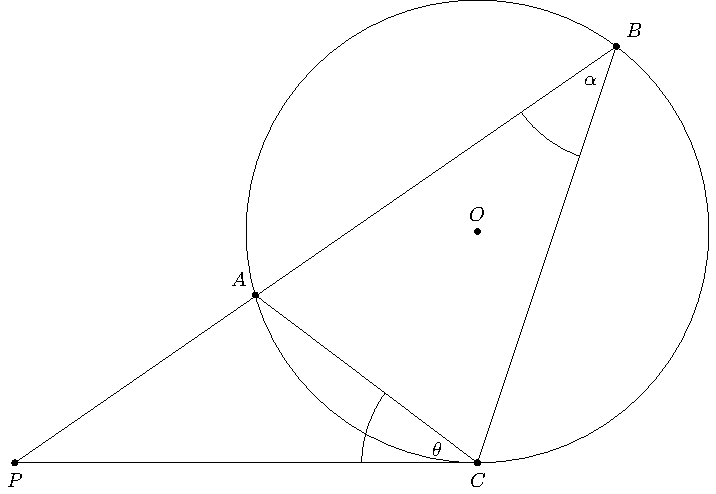
\includegraphics[width=0.6\columnwidth]{figs/trig_id/ccircle/circ_tang_icept.pdf}}
		\end{center}
		\caption{$\theta= \alpha$.}
		\label{fig:circ_tang_icept}	
	\end{figure}
\item
	In Fig. \ref{fig:circ_tang_icept}, show that $PA.PB = PC^2$.
\label{them:circ_tang_icept_prod}	
\\
\solution 
In $\triangle$s $APC$ and $BPC$, 
using
		\eqref{fig:circ_tang_icept-equal},	
  \begin{align}
	  \frac{AP}{\sin \theta} &= \frac{AC}{\sin P} 
	  \\
	  \frac{PC}{\sin \theta} &= \frac{BC}{\sin P} 
	  \\
	  \implies \frac{PC}{AP} &= \frac{BC}{AC}  \brak{= \frac{BP}{CP}}
  \end{align}
  which gives the desired result.
$\triangle$s $APC$ and $BPC$ are said to be {\em similar}.
\item  The perpendicular from the centre of a circle to a chord bisects the chord. 
\item  The line drawn through the centre of a circle to bisect a chord is perpendicular to the chord.
\end{enumerate}
%
